\chapter{Decaimiento del muón y espectro de Michel}\label{DEC_MUON_MICHEL}
\section{Decaimiento del muón}
	El muón, al igual que el electrón, se encuentra dentro del grupo de los leptones en el modelo estándar, ambos presentan características similares, tienen la misma carga y el mismo espín ($1/2$), pero la principal diferencia se encuentra en la masa, la masa del muón es aproximadamente 200 veces la masa del electrón y además es inestable, por consiguiente, el muón decae en un electrón y dos neutrinos,\\
	\begin{equation}
	\mu^{-} \rightarrow e^{-}+\Bar{\nu_{e}}+\nu_{\mu}
	\end{equation}
	con un tiempo de vida media de $\tau=(2.19698110\pm 0000022)\mu s$ \cite{Olive_2014}. Este decaimiento puede ser ilustrado mediante diagramas de Feynman como se muestra en la figura \ref{MUON_DECAY}.
	
	\begin{figure}[h]
		\centering
		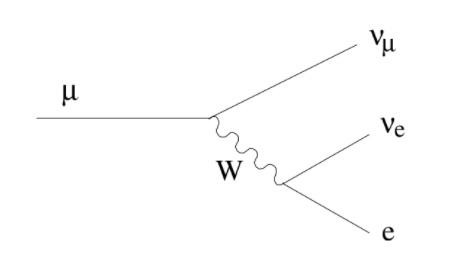
\includegraphics[scale = 0.65]{FIGURAS/MUON_DECAY.png}
		\caption{Proceso del decaimiento del muón.}
		\label{MUON_DECAY}
	\end{figure}

	Sin embargo en la naturaleza, y debido a las cascadas producidas por los rayos cósmicos primarios (ver sec.\ref{EAS}) se producen partículas muonicas positivas y negativas, lo que tiene un efecto al momento de medir su tiempo de decaimiento dentro de los tanques Cherenkov de agua. Los muones negativos, al momento de interaccionar con el medio (agua) va a sufrir lo que se conoce como captura muonica, lo que conlleva a que su tiempo de decaimiento sea menor, lo que no sucede con los muones positivos. Por ende, en los experimentos donde se desea obtener el $\tau$, éste va ser un promedio de ambos tiempo de vida media; entonces podemos decir que si nosotros logramos medir $\tau=2.196 \mu s$ nos indicaría que hay más presencia de muones positivos \cite{Holmlid}.
	
	El electrón que resulta del decaimiento del muón es conocido como electrón de Michel \cite{michel}. El análisis de la distribución de energía de estos electrones de Michel representa un punto de calibración en nuestros detectores Cherenkov, de esta manera, obtenemos un monitoreo continuo del funcionamiento y hasta del nivel de agua de los mismos \cite{ZUO20181}.

\section{Espectro de Michel}\label{ESPECTRO_MICHEL}
	El proceso en el que un muón decae en un electrón y dos neutrinos se le conoce a menudo como decaimiento Michel \cite{RENGA2019100029}. Debido a su corta energía, en promedio de 37 MeV y máximo 53 MeV, los electrones del Michel depositan toda su energía dentro de un tanque, por lo que la energía depositada en el tanque es independiente del nivel de agua \cite{ZUO20181}. Obtener un espectro de Michel (distribución energética de los electrones de Michel) puro es complicado experimentalmente ya que es casi imposible eliminar la contribución de los rayos cósmicos de fondo en dicho rango de energía, los rayos cósmicos de fondo es la radiación de fondo en la superficie que logra entrar al tanque y ser detectado por los PMT. Por lo tanto, para la obtención del espectro de Michel se suele recurrir a la simulación, ver figura \ref{MICHEL_ESPECTRO_SIMULADO}.
	
	\begin{figure}[h]
		\centering
		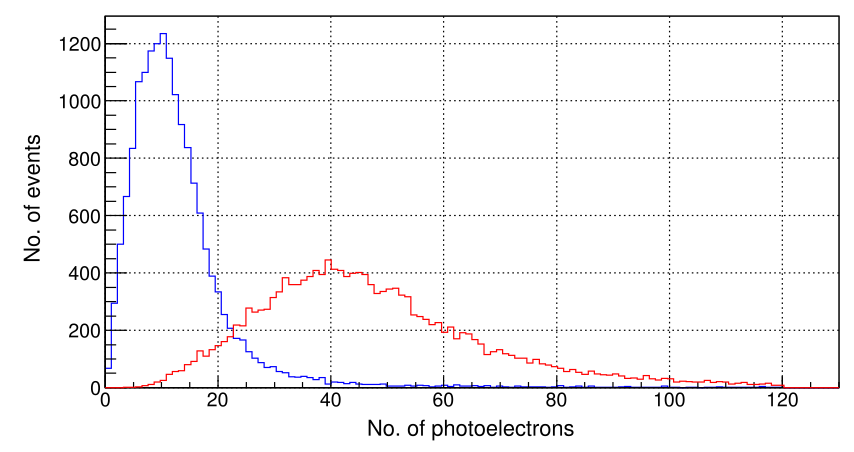
\includegraphics[scale = 0.45]{FIGURAS/ESPECTRO_MICHEL_SIMULADO.png}
		\caption{Distribución energética de los electrones de Michel (línea azul) y distribución energética de los muones frenados dentro del tanque (linea roja) \cite{ZUO20181}. Note que el número de fotoelectrones (eje X) es proporcional a la energía.}
		\label{MICHEL_ESPECTRO_SIMULADO}
	\end{figure}